% Conference-native artwork: figures are NOT scaled-down general-paper plates.
\newcommand{\FableFigure}{
\begin{figure*}[!t]
\centering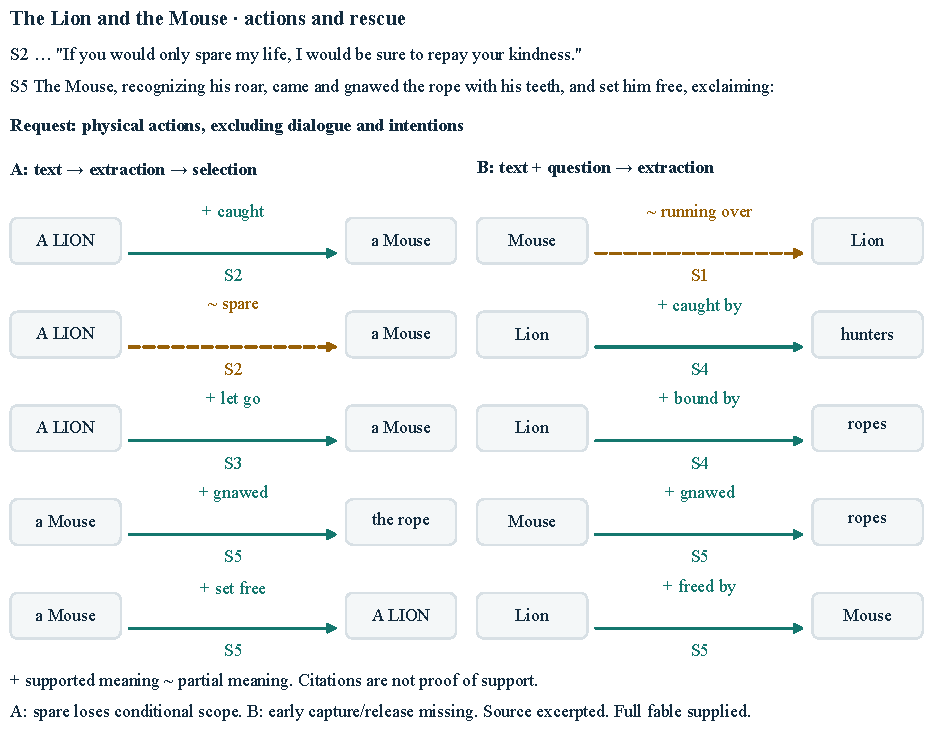
\includegraphics[width=0.95\textwidth]{figures/fable.pdf}
\caption{Fable action records from fixed selection (A) and contextual extraction (B). + marks supported meaning; $\sim$ marks partial meaning.}
\label{fig:fable}
\end{figure*}}
\newcommand{\OrchardFigure}{
\begin{figure*}[!t]
\centering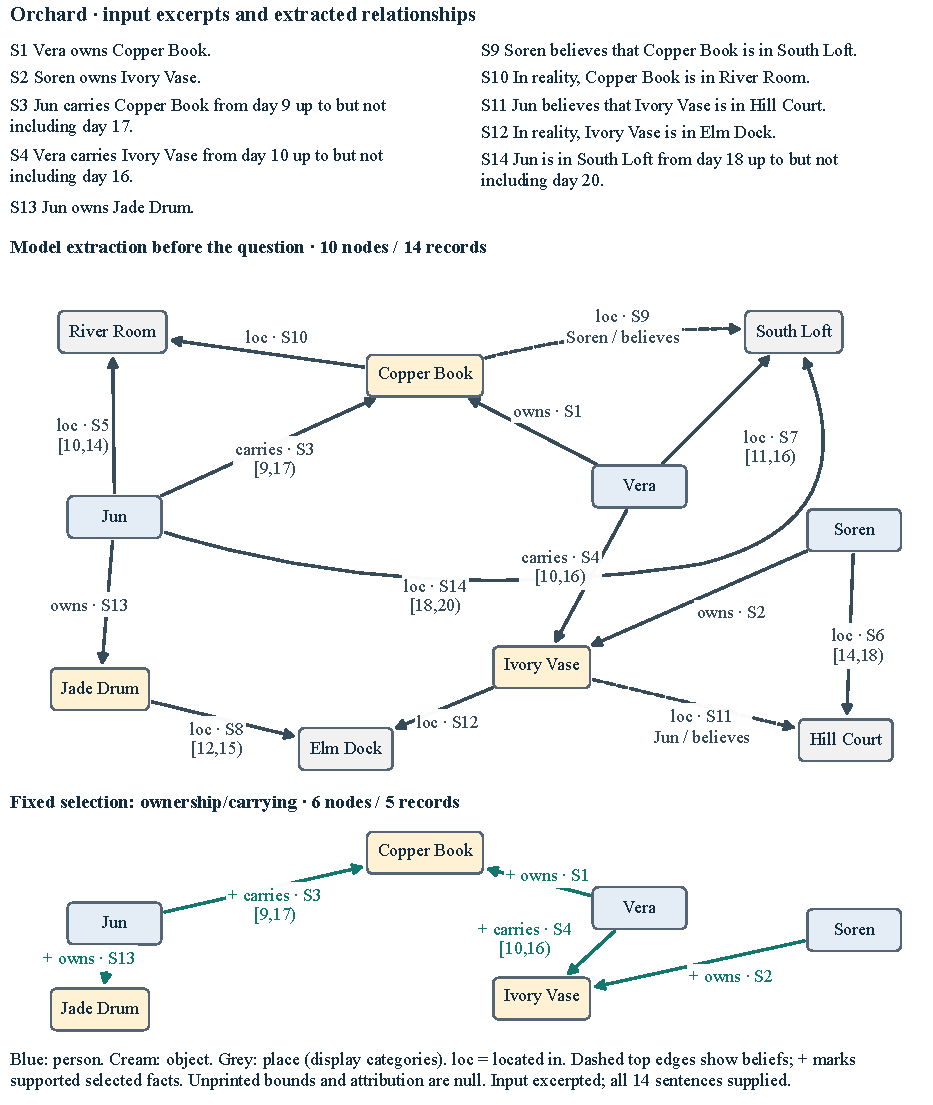
\includegraphics[width=0.95\textwidth]{figures/orchard_network.pdf}
\caption{Orchard input excerpts, model extraction (top network) and fixed ownership/carrying selection (bottom). Believer names qualify edges; they do not add relationships.}
\label{fig:orchard}
\end{figure*}}
\newcommand{\AliceFigure}{
\begin{figure*}[!t]
\centering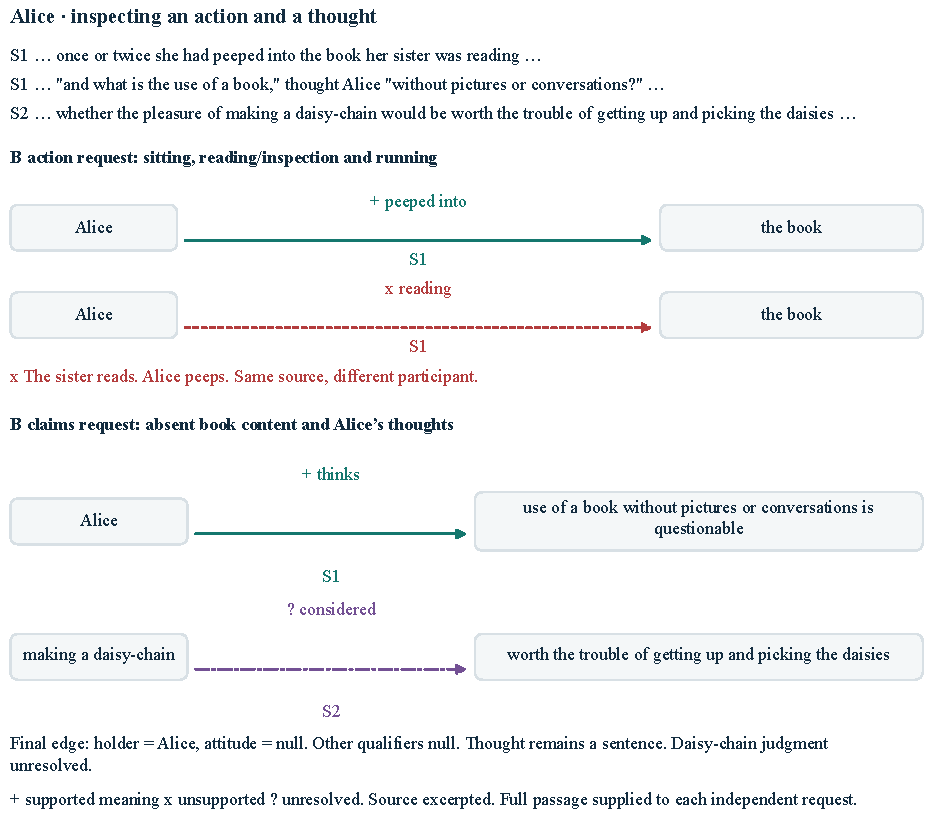
\includegraphics[width=0.95\textwidth]{figures/alice.pdf}
\caption{Alice's contextual action and thought records. + marks supported meaning, x a wrong participant, and ? an unresolved interpretation.}
\label{fig:alice}
\end{figure*}}
